%\tikzstyle{num} = [rectangle, minimum width = 0.6cm, minimum height = 0.6cm, text centered,align=center,thick,draw = black, fill = black!8]
\tikzstyle{num} = [rectangle, minimum width = 0.6cm, minimum height = 0.6cm, text centered,align=center,thick,draw = black,rounded corners=1.5pt]


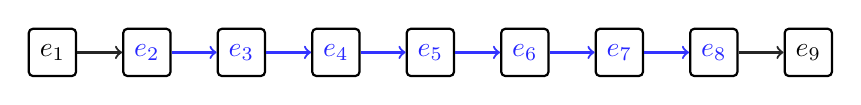
\begin{tikzpicture}[node distance = 0cm]
\node(num1)[num]{$\mathbi{e}_1$};
\node(num2)[num,right of = num1,xshift = 1.2cm]{\textcolor{blue!85}{$\mathbi{e}_2$}};
\node(num3)[num,right of = num2,xshift = 1.2cm]{\textcolor{blue!85}{$\mathbi{e}_3$}};
\node(num4)[num,right of = num3,xshift = 1.2cm]{\textcolor{blue!85}{$\mathbi{e}_4$}};
\node(num5)[num,right of = num4,xshift = 1.2cm]{\textcolor{blue!85}{$\mathbi{e}_5$}};
\node(num6)[num,right of = num5,xshift = 1.2cm]{\textcolor{blue!85}{$\mathbi{e}_6$}};
\node(num7)[num,right of = num6,xshift = 1.2cm]{\textcolor{blue!85}{$\mathbi{e}_7$}};
\node(num8)[num,right of = num7,xshift = 1.2cm]{\textcolor{blue!85}{$\mathbi{e}_8$}};
\node(num9)[num,right of = num8,xshift = 1.2cm]{$\mathbi{e}_9$};
%\node(A)[below of = num2,yshift = -0.6cm]{A};
%\node(B)[below of = num8,yshift = -0.6cm]{B};


\draw [->, thick, color = blue!80](num2.east)--(num3.west);
\draw [->, thick, color = blue!80](num3.east)--(num4.west);
\draw [->, thick, color = blue!80](num4.east)--(num5.west);
\draw [->, thick, color = blue!80](num5.east)--(num6.west);
\draw [->, thick, color = blue!80](num6.east)--(num7.west);
\draw [->, thick, color = blue!80](num7.east)--(num8.west);

\draw [->,thick,color = black!85] (num1) -- (num2);
\draw [->,thick,color =black!85] (num8) -- (num9);


\end{tikzpicture}